\documentclass[12pt]{article}

\usepackage[margin=0.5in]{geometry}
\usepackage{cite}
\usepackage{etoolbox}
\usepackage{graphicx}
\usepackage{hyperref}
\usepackage{wrapfig}

% https://tex.stackexchange.com/a/132647
\patchcmd{\thebibliography}{\section*{\refname}}{}{}{}


\begin{document}
\begin{center}
  {\Large TITLE}

  Michael Whittaker
\end{center}

In CS 186: Intro to Database Systems, students learn about the design and
implementation of relational databases: complex pieces of software that are
responsible for storing and managing data. One of the key challenges in
designing a database is ensuring that data is never lost, even if the database
crashes and later recovers. The de facto standard recovery algorithm that is
taught in nearly every undergraduate course on databases is ARIES, and let me
tell you, it's \emph{really} complicated. How complicated? Well, the original
paper that introduced ARIES is a whopping \textbf{69 pages}
long~\cite{mohan1992aries}! In it, the author notes that \emph{``concurrency
and recovery are complex subjects to think about and program for.''} The CS 186
textbook comments on ARIES saying that \emph{``the recovery manager is one of
the hardest components of a DBMS to design and
implement.''}~\cite{ramakrishnan2000database}. Due to its complexity, it's rare
to see a professor (or even a textbook) walk through a complete execution of
the algorithm, despite the fact that the algorithm is foundational and almost
always asked about on exams. As a result, students either spend an exorbitant
amount of time struggling to understand ARIES or flat out give up.

\begin{wrapfigure}{r}{0.5\textwidth}
  \centering
  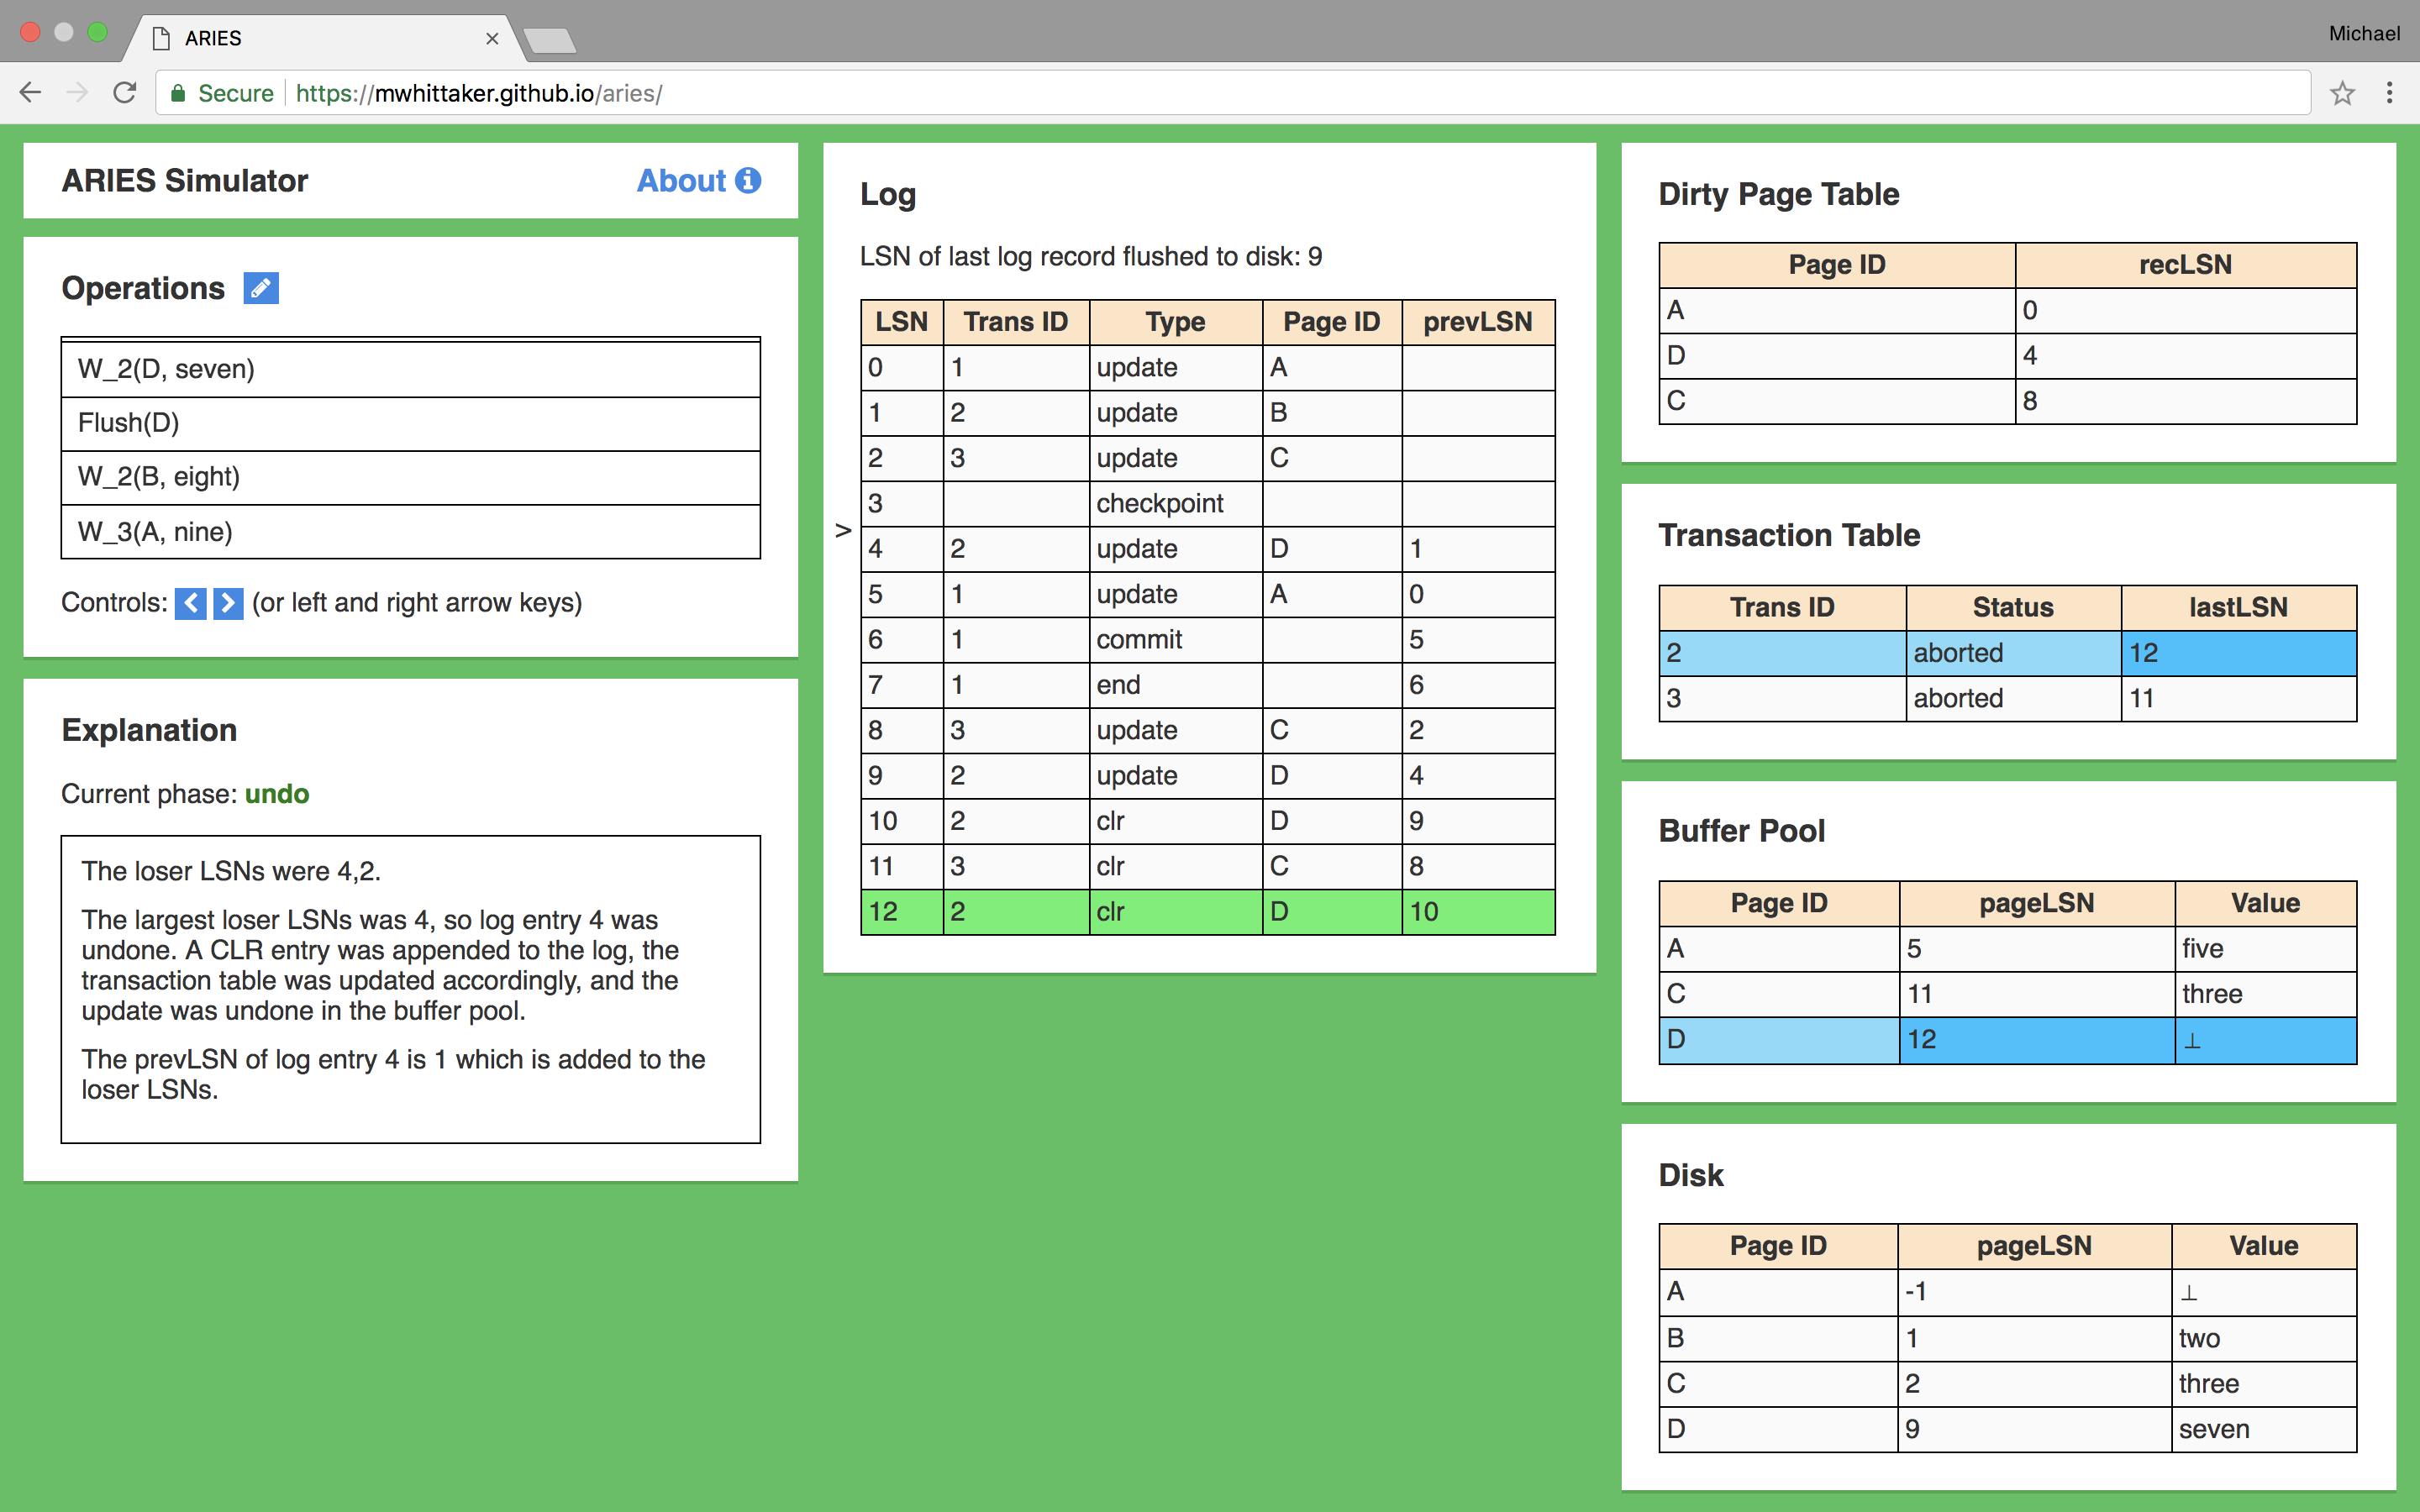
\includegraphics[width=0.5\textwidth]{aries.png}
  \caption{Online ARIES Simulator}\label{LarrysAries}
\end{wrapfigure}

To make it easier for students to learn ARIES, another CS 186 GSI (Larry Xu)
and I implemented the ARIES algorithm and an accompanying online visualization.
The visualization is depicted in Figure~\ref{LarrysAries} and can be found
online at \url{mwhittaker.github.io/aries}.
% TODO: Mention that students can run on arbitrary inputs.
% TODO: Mention that it comes with written explanations.
% TODO: Mention that students can read the source code.

% Evaluation
%   - "This is a really really high quality teaching tool IMO. Great job Michael and Larry! :)"
%   - count piazza questions? Analyze how many were answered with simulation
%   - github stars
%   - 935 page views, 443 users,

{
  \footnotesize
  \bibliographystyle{plain}
  \bibliography{references}
}
\end{document}
